% Part: model-theory
% Chapter: interpolation
% Section: separation

\documentclass[../../../include/open-logic-section]{subfiles}

\begin{document}

% SEGMENT OLP-0200-S01

\olfileid{mod}{int}{sep}

\olsection{\printtoken{P}{sentence}களைப் பிரித்தல்}

இடையீட்டுத் தேற்றத்தின் நிரூபிப்பைத் தொடர்வதற்கு முன் சில அடிப்படை
வேலைகள் தேவை. $!A$ மற்றும் $!B$ இன் இடையீட்டி என்பது
$!A \Entails !C$ மற்றும் $!C \Entails !B$ ஆகுமாறு !!a{sentence}~$!C$.
முரண்நிலைப்படி, பிந்தையது $\lnot !B \Entails \lnot
!C$ எனில், எனில் மட்டுமே, மெய். இப்பண்புடைய !!^a{sentence}~$!C$
ஆனது $!A$ மற்றும் $\lnot !B$ ஐ \emph{பிரிக்கிறது} எனப்படுகிறது.
எனவே $!A$ மற்றும் $!B$ க்கான இடையீட்டியைக் கண்டறிவது, $!A$ மற்றும்
$\lnot !B$ ஐப் பிரிக்கும் !!a{sentence} ஒன்றைக் கண்டறிவதற்குச் சமம்.
அடிக்கடி செய்வதுபோல, ஒரு பொதுமைப்படுத்தலைக் கருதுவது பயனுடையது:
!!{sentence}s இன் இரு \emph{கணங்களைப்} பிரிக்கும் ஒரு வாக்கியம்.

\begin{defn}
$\Gamma \Entails !C$ மற்றும் $\Delta \Entails
\lnot !C$ எனில், எனில் மட்டுமே, வாக்கியம் $!C$ ஆனது வாக்கியங்களின்
கணங்கள் $\Gamma$ மற்றும் $\Delta$ ஐ \emph{பிரிக்கிறது}. அத்தகைய
!!{sentence} இல்லையெனில், $\Gamma$ மற்றும் $\Delta$
\emph{பிரிக்கவியலாதவை}.
\end{defn}

$\Gamma$, $\Delta$, $!C$ ஆகியவற்றின் மாதிரி வகுப்புகளுக்கு இடையிலான
உள்ளடக்க உறவுகள் கீழே காட்டப்பட்டுள்ளன:
\begin{figure}[h]
  \centering
  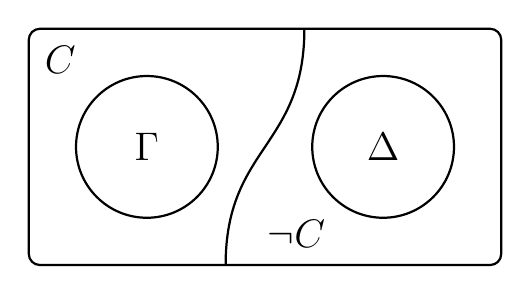
\begin{tikzpicture}[node distance=2cm, auto, thick]
    \draw [rounded corners] (0,0) -- (6,0) -- (6,3) -- (0,3) --  cycle;
    \draw (1.5,1.5) circle (0.9cm);
    \draw (4.5,1.5) circle (0.9cm);
    \path node at (1.5,1.5) {\Large $\Gamma$};
    \path node at (4.5,1.5) {\Large $\Delta$};
    \path node at (0.4,2.6) {\Large $\formula{C}$};
    \path node at (3.4,0.4) {\Large $\lnot \formula{C}$};
    \draw (2.5,0) .. controls (2.5,1.5) and (3.5,1.5) .. (3.5,3);
  \end{tikzpicture}
  \caption{$!C$ ஆனது $\Gamma$ மற்றும் $\Delta$ ஐப் பிரிக்கிறது}
  \ollabel{fig:sep}
\end{figure}


\begin{lem}\ollabel{lem:sep1}
$\Gamma$ மற்றும் $\Delta$ ஆகிய \emph{இரண்டிலும்} இடம்பெறும் ஒவ்வொரு
!!{constant}, !!{function}, !!{predicate} ஐயும் ($\doteq$ தவிர)
கொண்ட மொழி $\Lang{L}_0$ என்று கொள்க; மேலும் $n
\ge 0$ க்கான எண்ணிலடங்கா புதிய !!{constant}s $\Obj c_n$ ஐச்
சேர்ப்பதன் மூலம் $\Lang{L}'_0$ பெறப்படுகிறது என்று கொள்க. அப்போது
$\Gamma$ மற்றும் $\Delta$ ஆகியவை $\Lang{L}_0$ இல் பிரிக்கவியலாதவை
எனில், அவை $\Lang{L}'_0$ இலும் பிரிக்கவியலாதவை.
\end{lem}

\begin{proof}
மறைமுகமாகச் செல்கிறோம்: முரண்பாட்டிற்காக $\Gamma$ மற்றும் $\Delta$
ஆகியவை $\Lang{L}'_0$ இல் பிரிக்கப்படுகின்றன என்று கொள்க. அப்போது
ஏதேனும் $!C \in
\Lang{L}_0$ க்கு $\Gamma \Entails
\Subst{!C}{c}{x}$ மற்றும் $\Delta \Entails \lnot
\Subst{!C}{c}{x}$ (இங்கே $c$ ஒரு புதிய !!{constant}---$!C$ ஒன்றுக்கு
மேற்பட்ட அத்தகைய புதிய !!{constant} ஐக் கொண்ட நிலையும் இதே போன்றது).
இறுதிக்குட்பட்ட தன்மையின்படி,
$\Gamma_0 \Entails \Subst{!C}{c}{x}$ மற்றும்
$\Delta_0 \Entails \lnot \Subst{!C}{c}{x}$ ஆகுமாறு $\Gamma$ இன்
\emph{இறுதிக்குட்பட்ட} உட்கணம் $\Gamma_0$ உம் $\Delta$ இன்
உட்கணம் $\Delta_0$ உம் உள்ளன. $\Gamma_0$ இலுள்ள எல்லா
!!{formula}s இன் இணைப்பை $!G$ என்றும், $\Delta_0$ இலுள்ள எல்லா
!!{formula}s இன் இணைப்பை $!H$ என்றும் கொள்க. அப்போது
\begin{align*}
  !G & \Entails \Subst{!C}{c}{x}, & !H  \Entails \lnot \Subst{!C}{c}{x}.
\end{align*}
முந்தையதிலிருந்து பொதுமைப்படுத்தலால் $!G \Entails
\lforall[x][!C]$ கிடைக்கிறது; பிந்தையதிலிருந்து முரண்நிலைப்படி
$\Subst{!C}{c}{x} \Entails \lnot !H$; எனவே
$\lforall[x][!C]
\Entails \lnot \delta$ உம் கிடைக்கிறது. மீண்டும் முரண்நிலை
$!H \Entails
\lnot \lforall[x][!C]$ என்பதைக் கொடுக்கிறது. ஓரியக்கத்தன்மையின்படி,
\begin{align*}
  \Gamma &\Entails \lforall[x][!C], &
  \Delta & \Entails \lnot \lforall[x][!C],
\end{align*}
எனவே $\lforall[x][!C]$ ஆனது $\Lang{L}_0$ இல் $\Gamma$ மற்றும்
$\Delta$ ஐப் பிரிக்கிறது.
\end{proof}

\begin{lem}\ollabel{lem:sep2}
$\Gamma \cup \{ \lexists[x][!S] \}$ மற்றும் $\Delta$
பிரிக்கவியலாதவை என்றும், $c$ ஆனது $\Gamma$, $\Delta$, $!S$
ஆகியவற்றில் இல்லாத புதிய !!{constant} என்றும் கொள்க. அப்போது
$\Gamma \cup \{ \lexists[x][!S], \Subst{!S}{c}{x} \}$ மற்றும்
$\Delta$ உம் பிரிக்கவியலாதவை.
\end{lem}

\begin{proof}
ஒரே நேரத்தில் $\Gamma \cup \{\lexists[x]{!S} \}$ மற்றும் $\Delta$
பிரிக்கவியலாதவையாக இருக்க, $!C$ ஆனது
$\Gamma \cup \{
\lexists[x][!S], \Subst{!S}{c}{x}\}$ மற்றும் $\Delta$ ஐப் பிரிக்கிறது
என்று முரண்பாட்டிற்காகக் கொள்க. இரு நிலைகளை வேறுபடுத்துகிறோம்:
\begin{enumerate}
\item $!C$ இல் $c$ இடம்பெறவில்லை: இந்நிலையில்
$\Gamma \cup
  \{\lexists[x][!S], \lnot!C \}$ நிறைவுறத்தக்கது
(இல்லையெனில் $!C$ ஆனது $\Gamma \cup \{\lexists[x][!S] \}$ மற்றும்
$\Delta$ ஐப் பிரிக்கிறது). $\Subst{!S}{c}{x}$ ஐச் சேர்த்தாலும் அது
நிறைவுறத்தக்கதாகவே உள்ளது; எனவே இறுதியில் $!C$ ஆனது
$\Gamma \cup \{ \lexists[x][!S], \Subst{!S}{c}{x} \}$ மற்றும்
$\Delta$ ஐப் பிரிக்கவில்லை.
\item $!C$ இல் $c$ இடம்பெறுகிறது; எனவே $!C$ ஆனது
  $\Subst{!C}{c}{x}$ வடிவில் உள்ளது. அப்போது
  \[
  \Gamma \cup \{ \lexists[x][!S], \Subst{!S}{c}{x}\} \Entails \Subst{!C}{c}{x},
  \]
  என்று கிடைக்கிறது. இதிலிருந்து உய்த்தறிதல் தேற்றம் மற்றும்
  பொதுமைப்படுத்தலால்
  $\Gamma, \lexists[x][!S] \Entails \lforall[x][(!S \lif !C)]$;
  இறுதியாக $\Gamma
  \cup \{ \lexists[x][!S] \} \Entails \lexists[x][!C]$. மறுபுறம்,
  $\Delta \Entails \lnot \Subst{!C}{c}{x}$; எனவே
  பொதுமைப்படுத்தலால் $\Delta \Entails \lnot \lexists[x][!C]$.
  ஆகவே $\Gamma
  \cup \{\lexists[x][!S] \}$ மற்றும் $\Delta$ பிரிக்கத்தக்கவை;
  இது முரண்பாடு.
\end{enumerate}
\end{proof}

\end{document}
